\section*{System Demonstration}
\label{sec:demo}

\begin{figure*}[!t]
  \centering
  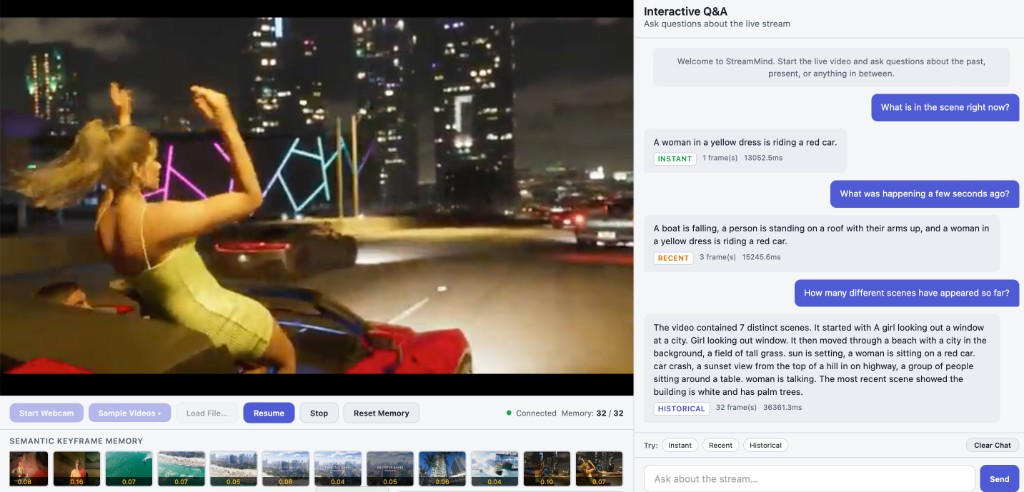
\includegraphics[width=\linewidth]{figures/demo_screenshot.png}
  \caption{\textbf{StreamMind live demo.} The interface shows a GTA~VI trailer playing in the video panel (left) with the SKM filmstrip and per-frame importance scores below it (Memory: 32/32). The chat panel (right) displays three queries spanning all temporal scopes: an \textsc{instant} query identifies the current scene, a \textsc{recent} query describes events from the last few seconds, and a \textsc{historical} query summarises all seven distinct scenes encountered so far. Each response includes its classified scope, the number of context frames used, and the end-to-end latency.}
  \label{fig:demo}
\end{figure*}

We provide a live web demo (\Cref{fig:demo}) that lets users interact with \ours through a browser.
A FastAPI backend runs the full CLIP + BLIP + Flan-T5 pipeline and communicates with the front end over WebSockets.
The interface splits into two panels.
The \emph{video panel} (left) shows the live feed together with the SKM filmstrip: each thumbnail displays its importance score, and the memory counter tracks the current fill level against the configured capacity.
The \emph{chat panel} (right) accepts free-form questions and returns answers annotated with the classified temporal scope, the number of keyframes consulted, and per-query latency.
Users can stream from their webcam, upload a local video file, or choose from pre-loaded sample clips including movie trailers and activity montages.

A dedicated \emph{workshop presentation mode} enlarges all UI elements for projector visibility and offers one-click sample questions that step through all three temporal scopes, letting the presenter walk the audience through the pipeline interactively.
We plan to present a live demo at the workshop, allowing attendees to ask questions about a live webcam feed and observe the SKM, TQR, and SFG components operating in real time.

The demo runs on GPU or CPU (1--3\,s per query on CPU, $<$200\,ms on A100) and ships with a Docker configuration for one-command startup (\texttt{docker compose up}).
All source code, the LiveQA-Bench dataset, evaluation scripts, and the interactive demo are publicly available at \url{https://github.com/palsure/StreamMind-LiveQA}.
